\documentclass[11pt]{article}
\RequirePackage{fullpage}
%\RequirePackage[font=small,labelfont=bf]{caption}
\RequirePackage{amsmath,amssymb,amsthm}
\RequirePackage{graphicx}
\RequirePackage[hidelinks]{hyperref}
\RequirePackage{subcaption}
\RequirePackage{wasysym}
\RequirePackage{authblk}
\RequirePackage{bm}
\RequirePackage{bbm}

\RequirePackage{cleveref}
\RequirePackage{xr}

\newcommand*{\addFileDependency}[1]{
\typeout{(#1)}

\IfFileExists{#1}{}{\typeout{No file #1.}}
}\makeatother

\newcommand*{\myexternaldocument}[1]{%
\externaldocument{#1}%
\addFileDependency{#1.tex}%
\addFileDependency{#1.aux}%
}

\myexternaldocument{supplementary}


%\RequirePackage[osf]{mathpazo}
\let\temp\rmdefault
\RequirePackage{mathpazo}
\let\rmdefault\temp

\RequirePackage[bibstyle=authoryear,citestyle=authoryear-comp,
                date=year,
                maxbibnames=9,maxnames=5,maxcitenames=2,
                backend=biber,uniquelist=false,uniquename=false,
                % style=apa,
                sorting=nyt,
                % sorting=,
                hyperref=true]{biblatex}
\RequirePackage{color}
\RequirePackage{nicefrac}

\addbibresource{biblio.bib}

% line numbers:
\RequirePackage[left, modulo]{lineno}
\modulolinenumbers[2]

% spacing
\RequirePackage{setspace}
\onehalfspacing


\renewcommand{\P}{\mathbb{P}}
\newcommand{\E}{\mathbb{E}}
\newcommand{\V}{\text{V}}
\DeclareMathOperator{\var}{var}
\DeclareMathOperator{\cov}{cov}


%\title{Towards a Complete Model of the Negative Selection Process in Humans}
%\title{An Evolutionary Quantitative Genetic Model of the Negative Selection Process in Humans}
\title{A Quantitative Genetic Model of Background Selection in Humans}

\author[1,2,$\dag$]{Vince Buffalo}
\author[2]{Andrew D. Kern}
\affil[1]{\small{Department of Integrative Biology, University of California, Berkeley}}
\affil[2]{\small{Institute of Ecology and Evolution and Department of Biology, University of Oregon }}
\affil[*]{Corresponding author email: \href{vsb@berkeley.edu}{vsb@berkeley.edu}}


\begin{document}
\maketitle

\linenumbers
\begin{abstract}
    Across the human genome, there are large-scale fluctuations in genetic diversity caused by the indirect effects of selection. 
    This ``linked selection signal" reflects the impact of selection according to the physical placement of functional regions and recombination
    rates along chromosomes. Previous work has shown that purifying selection
    acting against the steady influx of new deleterious mutations at functional portions
    of the genome shapes patterns of genomic variation. To date, statistical
    efforts to estimate purifying selection parameters from linked selection models have relied on
    classic Background Selection theory, which is only applicable when new mutations are so deleterious that they cannot fix in the population. 
    Here, we develop a statistical method based
    on a quantitative genetics view of linked selection, that models how
    polygenic additive fitness variance distributed along the genome increases 
    the rate of stochastic allele frequency change. By 
    jointly predicting the equilibrium fitness variance and substitution rate
    due to both strong and weakly deleterious mutations, we estimate the
    distribution of fitness effects (DFE) and mutation rate across three geographically distinct human samples. While our model can accommodate weaker selection, we find evidence of strong selection operating similarly across all human samples. While our quantitative genetic model of linked selection fits better than previous models, substitution rates of the most constrained sites are poorly predicted. We find evidence that a model incorporating selective interference better predicts observed divergence, but overall our results ultimately suggest considerable uncertainty remains about the processes generating fitness variation in humans.
\end{abstract}


\section*{Introduction}

The continual influx of new mutations into populations is the ultimate source of all adaptations, but the vast majority of mutations either do not affect fitness or are deleterious. Natural selection works to eliminate these deleterious mutations from the population, thus we expect them to appear at low frequencies within populations \parencite{Haldane1927-ga}, and be less likely to fix between lineages. Conserved genomic regions reflect the product of hundreds of millions of years of evolutionary optimization; thus the overwhelming majority of segregating variation in these regions will have deleterious fitness effects. Consequently, a good predictor of whether a new mutation will reduce fitness is if it occurs in a region of the genome that has been conserved over phylogenetic timescales \parencite{Siepel2005-wh,Margulies2003-sn}. Moreover, segregating rare variation in these regions is responsible for a significant proportion of the genetic contribution to phenotypic variation and disease in humans\parencite{Zeng2018-ci,Lek2016-cb,Karczewski2020-ky,Tennessen2012-ge}.

Selection on both beneficial and deleterious variants perturbs the allele frequencies of neighboring linked sites, a phenomenon known as linked selection
\parencite{Nordborg1996-nq,Maynard_Smith1974-zr,Barton1998-aj,Charlesworth1993-gb,Kaplan1989-sc}.
Since deleterious variation is clustered in functional portions of the genome,
we expect linked selection to reduce levels of diversity around evolutionarily constrained
segments (e.g. genes, regulatory elements, etc.). The genomic arrangement of
these evolutionarily conserved regions coupled with heterogeneous recombination rates create a
large-scale spatial signal of linked selection of genetic diversity along chromosomes. Since genome-wide recombination maps and functional annotations are available for many species, there has been consistent effort to fit models of linked selection to patterns of diversity. This general approach provides estimates of population genetic
parameters such as the strength of selection and the deleterious mutation rate
\parencite{Hudson1995-pt,McVicker2009-ax}, and potentially distinguishes the roles of positive and negative selection and estimate the rate of
beneficial mutations \parencite{Elyashiv2016-vt,Murphy2022-sj}. In humans,
previous work has shown that negative selection plays the dominant role in
shaping megabase-scale patterns of diversity, with positive selection having a
nearly negligible impact \parencite{Murphy2022-sj}.

Prior work to model the reduction in linked diversity due to deleterious
mutations has largely relied on the classic Background Selection (BGS) model
\parencite{Charlesworth1993-gb,Nordborg1996-nq,Hudson1995-pt,Hudson1995-xc}.
While the BGS model has been successful in fitting many patterns of diversity,
some of its simplifying assumptions may distort inferences about the selective process. First, since fixation probabilities ultimately depend on the
product of the deleterious selection coefficient ($s$) and population size
($N$), the efficacy of selection depends on past population sizes.
Unfortunately, accommodating such demography into purifying selection models remains an open, difficult problem \parencite{Zeng2013-ep,Johri2020-oj}.
Second as the BGS model builds off classic models of mutation-selection balance
\parencite{Crow1970-wm,Kimura1966-bk}, it assumes that new mutations are sufficiently deleterious that they are invariably driven to loss. Under
this assumption, the effect of selection is well-approximated by simply
rescaling the neutral coalescent by a reduction factor known as $B =
\nicefrac{N_e}{N}$ \parencite{Charlesworth2013-kl}. However, this simple
rescaling approach is not appropriate across parts of parameter space that are
relevant to natural populations \parencite{McVean2000-bt,Good2014-yz}. In
particular, the BGS model cannot accommodate the possibility of weakly deleterious mutations (those with fitness effects $2Ns \le 1$) reaching fixation, which leads to incorrect
predictions of diversity levels as the strength of selection diminishes. 
Finally, the classic BGS
model assumes that the selective dynamics occurring within a segment are not impacted by selection occurring outside the segment, i.e. no selective or
``Hill--Robertson" interference
\parencite{Hill1966-kd,McVean2000-bt,Felsenstein1974-xm}.

In this work, we use another class of linked selection models that derive from
quantitative genetics to address limitations of the classic BGS model \parencite{Santiago1998-bs, Santiago2016-mu,Santiago1995-hx,Robertson1961-ho}.
These models consider how polygenic fitness variance spread along the genome increases the variance of stochastic allele frequency change, as alleles become randomly linked to fitness backgrounds over time and their frequency trajectories are perturbed by selection at other sites. While these models can theoretically accommodate additive fitness variance from any source as long as its rate of change is not too rapid, we focus
specifically on a deleterious-mutations-only model of fitness variance from
\textcite{Santiago2016-mu}. This model is identical to BGS when selection
against deleterious mutations is strong, but it also correctly predicts the
reduction in diversity when selection is weak by jointly predicting the
deleterious substitution rate. We extend the Santiago and Caballero (hereafter
the SC16) model of the negative selection process so that it can be fit using a composite likelihood approach to patterns of genome-wide diversity, according to the spatial distribution of genomic features that could harbor deleterious fitness variation. Using forward simulations, we show this model leads to more accurate estimates of the distribution of fitness effects (DFE) under weak selection. We apply our
composite-likelihood method to human population genomic data and provide new
parameter estimates of the genome-wide impact of purifying selection in humans. 
We show that our new method is better able to predict the patterns of diversity along human chromosomes than previous models. 
However, our model leads to predictions of the deleterious substitution rate that disagree with observed levels of divergence. We discuss the potential causes and implications of such discrepancies and what it might mean for future efforts to fit linked selection models to genomic patterns of variation.

\section*{Theory}

Our work extends quantitative genetic models of linked selection
\parencite{Robertson1961-ho,Santiago1995-hx,Santiago1998-bs,Santiago2016-mu},
which model the effects of linked selection in terms of polygenic additive fitness
variance ($V_A$). Here we review the relevant theory before introducing our genome-wide extension. These linked selection models stem from
\textcite{Robertson1961-ho}, which in essence describes how polygenic additive
fitness variation increases the pace of stochastic allele frequency change, thus reducing effective population size. At the individual level Robertson considered, 
selection generates an autocorrelation in fecundity as offspring from large
families tend to beget many descendants themselves (and likewise with small
families) when fitness is heritable. This same across-generation autocorrelation occurs at the
genomic level due to linkage \parencite{Santiago1998-bs,Barton2000-zg}, as the
perturbations to a neutral allele's trajectory from its particular fitness
background tend to occur in the same direction across generations until the
background recombines off. Quantitative genetic models such as \textcite{Santiago1998-bs}
quantify the total impact of the autocorrelation generated by selection in terms of what we think of as a
\emph{fitness-effective} population size $N_f$ (to differentiate it from the \emph{drift}-effective population size, which is the size of the ideal population when there is no fitness variation).

The key insight is that in the long run, the steady presence of additive genetic fitness variance ($V_A > 0$) contributes an extra source of variance in offspring number beyond the variance expected under pure drift \parencite{Wright1938-tv}. However, because heritable fitness variation generates across-generation autocorrelation, the cumulative effect of this fitness variance on the variance in allele frequency change is inflated by a factor of $Q^2$. Intuitively, the product $V_A Q^2$ represents the expected
total variance in reproductive success a neutral mutation experiences over its lifetime in a system with weak selection at linked sites. 

Following \textcite{Robertson1961-ho} and \textcite{Santiago1995-hx}, we define
the fitness-effective population size $N_f$ by including the total additional
variance created by heritable fitness into Wright's (\citeyear{Wright1938-tv})
equation for effective population size,

\begin{align}
    \label{eq:main_Ne}
    N_f = \frac{N}{Q^2 V_A + 1}
\end{align}
%
(c.f. \cite{Robertson1961-ho,Santiago1995-hx}; see Supplementary Materials Section
\ref{supp:theory} for a proof). The benefit of modeling linked selection with Robertson's
forward-time model is that the inflation factor is invariant with respect to the particular fitness background the neutral allele becomes stochastically associated with. By contrast,  modeling diversity levels under linked selection backwards in time requires tracking the particular associated fitness backgrounds, as coalescence rates experienced by a lineage are not invariant with respect to their fitness background.

Equation \eqref{eq:main_Ne} is general, since different modes of selection and
linkage can be accommodated by different expressions for $V_A$ and the
inflation factor $Q^2$ \parencite{Santiago1995-hx,Santiago1998-bs}. When
fitness variation has a multiplicative polygenic basis, as is often assumed for
genome-wide selection processes, the fitness-effective
population size experienced by an arbitrary neutral site under the influence of
all $S$ linked regions is,

\begin{align}
    \label{eq:polygenic_Ne}
    N_f \approx N \exp\left(-\sum_{i=1}^S V_{A,i} \frac{Q_i^2}{2}\right)
\end{align}
%
where the factor of one-half comes from ignoring the short-lived 
associations with the homologous chromosome, 
which have a weak effect on the focal allele (see Supplementary Materials Section
\ref{supp:heritable-fitness}). In our genome-wide model, we consider the
summation in Equation \eqref{eq:polygenic_Ne} over non-overlapping segments $i
\in \{1, 2, \ldots, S\}$ each undergoing selection such that segment $i$
contributes additive fitness variance $V_{A,i}$ to the total additive genetic
fitness variance. The impact this segment's fitness variance $V_{A,i}$ has on 
the fitness-effective population size is mediated by the autocorrelation term 
$Q_i$, which is a decaying function of the recombination rate between the 
segment and focal neutral allele. Specifically, the autocorrelation function
for a neutral allele associated with segment $i$ is $C(t) = [(1-r_i)(1-\kappa_i)]^t$, 
where $r_i$ is the recombination fraction to the segment and $\kappa_i$ is the rate that the
associated fitness variance decays due to selective dynamics. Then, the
cumulative autocorrelation over the lifespan of the allele is,

\begin{align}
    \label{eq:Q}
    Q_i &= 1 + \sum_{j=1}^\infty \left[(1-r_i)(1-\kappa_i)\right]^j \nonumber \\
        &= \frac{1}{\kappa_i + r_i(1-\kappa_i)}.
\end{align}
%
(see Supplementary Materials Equation \ref{supp-eq:Qinf}). This general equation can accommodate models of polygenic selection as long as the equilibrium additive fitness variation $V_{A,i}$ can be specified and the change in variance due to selection can be approximated as a geometric decay, i.e. $\Delta V_{A,i} = -\kappa V_{A,i}$ \parencite{Bulmer1971-ae,Keightley1988-eq,Walsh2018-bt, Santiago1998-bs}. This is usually a reasonable assumption since within-generation selection removes a fraction of phenotypic variation from the population, and some fraction of that is additive genetic variation \parencite{Bulmer1971-ae,Keightley1988-eq}.

The remaining required expressions are for the equilibrium additive fitness
variance $V_A$ and the decay rate in associated fitness $1-\kappa$. Fitness
variance could arise from beneficial or deleterious alleles, but given
prior work has found selection against new deleterious mutations in conserved regions plays a dominant role in shaping genome-wide patterns of diversity \parencite{McVicker2009-ax,Murphy2022-sj}, we focus specifically on purifying selection. We imagine a mutation-selection process that creates fitness variation as deleterious mutations enter a population at rate
$\mu$ per basepair per generation in a conserved region of $L$ basepairs, such
that the region-wide per generation diploid mutation rate is $U = 2 \mu L$.
Each mutation imposes a selective cost of $s$ in heterozygotes and $2s$ in
homozygotes, and fitness effects are multiplicative across sites. 

Under this selection model, the additive genic fitness variance created by a
new mutation (at frequency $x=\nicefrac{1}{2N}$) is $2s^2 x(1-x) \approx
\nicefrac{s^2}{N}$. For the entire population of $2N$ chromosomes, the mutational variance input each generation in segment $i$ is $V_{M,i} \approx
U_is^2$ where $U_i = 2\mu L_i$ is the diploid mutation rate per generation
within the segment. Under the mutation-selection balance assumed by classic BGS
theory, an $L_i$-basepair segment has equilibrium genic variance $V_{a,i}^{BGS}
\approx U_i s$ (see Supplementary Materials Equation \ref{supp-eq:va_bgs}) and
thus $\kappa_i^{BGS} = s$. Substituting $V_{a,i}^{BGS}$ and $\kappa_i^{BGS}$ in
Equation \eqref{eq:polygenic_Ne} and simplifying, we have

\begin{align}
    N_f = N \exp \left( - \sum_i^S \frac{\mu L_i}{s(1 + r_i(1-s)/s)^2} \right) 
\end{align}
%
which is identical to the genome-wide model of background selection used in
previous studies \parencite{McVicker2009-ax,Elyashiv2016-vt,Murphy2022-sj}.
Thus, the classic background selection model is a special case of the more
general theory of Santiago and Caballero (\citeyear{Santiago2016-mu}), which
they had shown previously (\citeyear{Santiago1998-bs}).

However, when new mutations are only weakly deleterious, they can drift up in
frequency before their eventual loss or fixation. At this point, the number of
deleterious mutations per haplotype is no longer well-approximated by the
deterministic mutation-selection-balance theory, and their dynamics are strongly
influenced by stochastic perturbations due to both drift and linked selection. 
In this weak selection regime, classic BGS theory no longer accurately predicts levels of linked diversity
\parencite{Charlesworth1993-gb,McVean2000-bt,Good2013-lp,Gordo2002-dr}.
Moreover, selection against weakly deleterious mutations alters the topology of genealogies, such that they are no longer well-approximated by a rescaled
neutral coalescent as assumed under the classic BGS model
\parencite{Przeworski1999-mb,OFallon2010-my,Higgs1995-xc}. To further
complicate matters, the distribution of the number of deleterious mutations
(and its corresponding fitness distribution) is no longer a stationary Poisson distribution, instead becoming a traveling wave
\parencite{Rouzine2008-qz,Good2013-lp,Gessler1995-hz} towards increased numbers
of deleterious alleles per chromosome and reduced mean population fitness.
In asexual populations, substitutions correspond to a click of ``Muller's ratchet", which is 
the stochastic loss of the least-loaded class \parencite{Muller1964-ki,Charlesworth1997-qn}.
Unfortunately, determining the rate of Muller's ratchet is another difficult problem
\parencite{Haigh1978-gt,Gordo2002-dr,Gessler1995-hz,Higgs1995-xc} related to
Hill--Robertson interference \parencite{Felsenstein1974-xm}.

Under quantitative genetic models of linked selection, these complications can
be avoided by finding a general expression for the equilibrium $V_A$ applicable
to both strong and weakly deleterious mutations while concurrently modeling the rate
of fixation of deleterious alleles in the region, $R$. \textcite{Santiago2016-mu}
suggest that equilibrium fitness variance is lower than predicted by
$V_{a}^{BGS}$ once weakly deleterious mutations begin to have an appreciable
rate of fixation $R > 0$ per generation in the region. The substitution rate $R$
decreases fitness variance since each substitution removes a segregating site 
and thus its contribution to fitness variance. Thus the steady-state additive 
genetic variance of fitness under mutation and negative selection is
(omitting the segment index $i$ for clarity),

\begin{align}
  \label{eq:Va}
  V_{a} = (U - 2 R)s. 
\end{align}

where the condition $V_a \ge 0$ is met when the probability of fixation is less
than or equal to the neutral fixation probability of $\nicefrac{1}{2N}$, as is true for all deleterious mutations. This equation describes the
equilibrium additive genetic fitness variance as the balance of the flux of new variation in to the population from deleterious mutations, and the removal of variation due to their substitution (and the decline in mean population fitness). When $R=0$, selection is so strong deleterious alleles cannot fix, and the equilibrium fitness variation is due entirely to young rare mutations before their extinction $V_a = V_a^{BGS} \approx Us$. Santiago and
Caballero derive Equation \eqref{eq:Va} through Fisher's Fundamental Theorem of
Natural Selection, but we find an alternative proof (\cite{Higgs1995-xc}; see
Supplementary Materials Section \ref{supp:weak-strong}). We also find that the
steady-state additive genic variance in Equation \eqref{eq:Va} results from
diffusion models with a flux of mutations into discrete sites
(\cite{Kimura1969-jw}). 

While using Equation \eqref{eq:Va} in Equation \eqref{eq:main_Ne} leads to a
prediction for the fitness-effective population size $N_f$, closed-form
expressions for the deleterious substitution rate $R$ have generally been hard to find
\parencite{Haigh1978-gt,Higgs1995-xc,Gessler1995-hz}. A key insight of
\textcite{Santiago2016-mu} is that the deleterious substitution rate with linked selection is determined by the probability of fixation $p_F(N_f, s)$
\parencite{Kimura1962-su,Malecot1952-qh} using the rescaled fitness-effective
population size, i.e. $R = N U p_F(N_f, s)$. Given this equation for the
substitution rate and Equation \eqref{eq:polygenic_Ne} for $N_f$ under linked selection, we have a
system of two non-linear equations that can be solved numerically for $N_f$ and
$R$ for each segment,

\begin{align}
  \label{eq:main_eqns}
  N_f &= N \exp \left( -(U-R)s \frac{Q^2}{2} \right) & \text{\emph{fitness-effective population equation}} \\
  R &= \frac{4N_f U s}{\exp(4 N_f s)-1}  & \text{\emph{substitution rate equation}}
\end{align}
%

We denote the solutions to these equations, which represent equilibria under
mutation-selection-drift process, as $\widetilde{N}_f$ and
$\widetilde{R}$. These equilibria also imply an equilibrium level of additive
fitness variation $\widetilde{V}_a$ in the segment, which are used to calculate
the reduction factor $B(x) = \nicefrac{N_f}{N}$ at any genomic position $x$
(see Methods Section \nameref{sec:methods-maps}).

\section*{Results}

We provide two main classes of results. First, we show simulation results which demonstrate
the accuracy of the SC16 model over the BGS approximation across the parameter space,
as well as validations of the composite likelihood strategy we use to fit the SC16 model. Second, we provide fits of our method to human genome data, where we show comparison of models fit using different annotations, the estimated DFEs, and predictions of the deleterious substitution
rate.

\subsection*{Simulation Validation of Theory and Methods}

Given that modeling the interplay of mutation, drift, and linked selection under both weak and strong selection has proven to be a difficult problem, we first sought to verify the SC16 theory and our genome-wide extension with three
levels of simulations: forward simulations of purifying selection in a region,
chromosome-scale forward simulations of purifying selection, and simulations of
a ``synthetic genome" (i.e. by combining independently simulated chromosomes) to test our composite-likelihood method based on this
theory.

\subsubsection*{Simulations of a Segment under Purifying Selection}
\label{sec:segment-sims}

\begin{figure}[htbp] \centering
    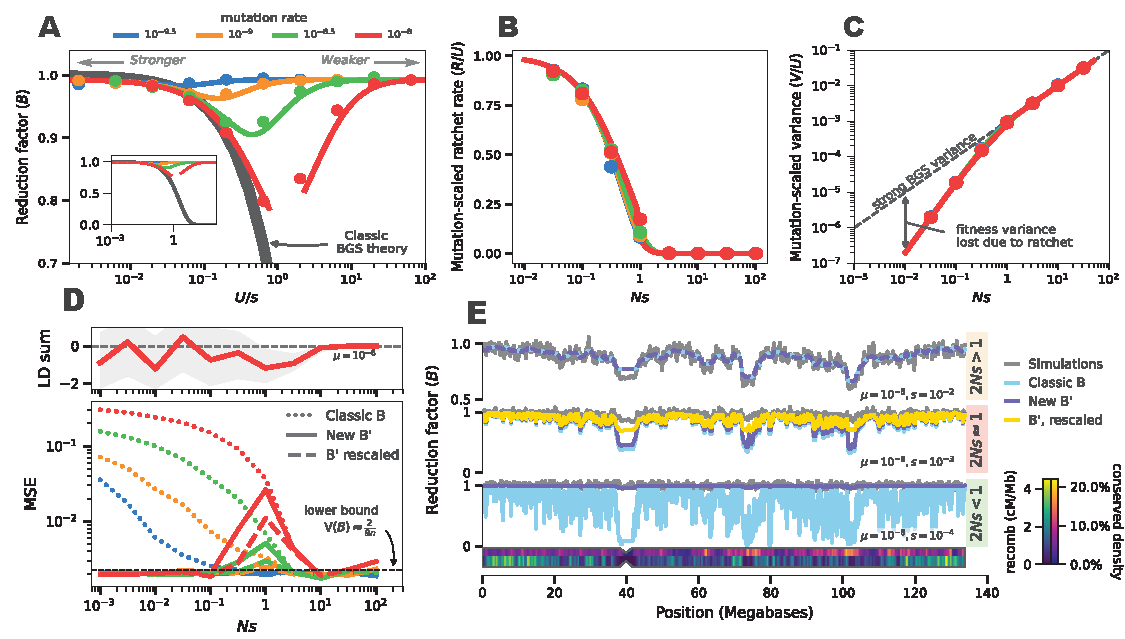
\includegraphics[width=\textwidth]{figures/figure_1.pdf} \caption{Santiago and Caballero (2016) theory models the weak selection regime better than classic BGS theory. (A) The predicted reduction factor
        under classic B theory (dark gray line) and the diploid SC16 model
        (colored lines corresponding to mutation rate) compared to average
        reduction across 10,000 simulation replicates (points). The inset figure is zoomed out to show extent of disagreement under classic BGS. (B) The predicted
        deleterious substitution rate under the SC16 model, scaled by mutation rate (colored
        lines) compared to the substitution rate estimated from simulation (points). When
        $2Ns>1$, the substitution rate is near zero. (C) The genic variance from
        simulations (points) against the predicted variance under the SC16
        model (colored lines). As substitutions begin to occur, the genic
        variance is decreased from the level expected under strong BGS (dashed
        line). (D, bottom) The mean squared error (MSE) between
        whole-chromosome simulations and predicted classic B (dots), new B'
        (solid), and locally rescaled B' (dashed) for different mutation rates
        (colors). Locally rescaled B' (yellow lines) are omitted for clarity in the top and bottom 
        rows, since they are identical to B'; Local rescaling only impacts B'
        in the $2Ns \approx = 1$ domain. The dashed horizontal line is the approximate theoretic
        minimum MSE. (D, top) The build-up of negative linkage disequilibria
        around $2Ns=1$ in whole-chromosome simulations shown in the bottom panel. (E) The
        average B map from 100 chromosome 10 simulation replicates (gray)
    against different predictions, for parameters that correspond to $2Ns < 1$,
$2Ns = 1$, and $2Ns > 1$. The chromosome shows the density of conserved sites
and recombination map used in simulations. }
  \label{fig:figure-1}
\end{figure}

Our first set of forward simulations was to ensure that the SC16 model
adequately captures selective dynamics in a single $100$ Mbp basepair region
under selection, across a variety of mutation rates and selection
coefficients (see Methods \nameref{sec:methods-sim}). We find a close
correspondence between the observed and predicted reductions in effective
population size $B=\nicefrac{N_f}{N}$ over all selection and mutation
parameters including weak selection (Figure \ref{fig:figure-1}A), in contrast
to classic BGS theory. Furthermore, to investigate whether this accuracy was
caused by the model correctly predicting the equilibrium fitness variance and
substitution rate, we also measured these throughout the simulation. Again, we find
diploid SC16 theory accurately predicts both the deleterious substitution rate (Figure
1\ref{fig:figure-1}B) and the genic fitness variance (Figure
1\ref{fig:figure-1}C).

Moreover, these simulations provide intuition about the underlying 
selection process. When mutations are strongly deleterious, there is no chance
they can fix, and the substitution rate is zero (Figure \ref{fig:figure-1}B for $2Ns
> 1$). In this strong selection regime, the additive genic fitness variation
closely matches the theoretic deterministic equilibrium of $V_a = Us$ (dashed
gray line, Figure \ref{fig:figure-1}C) However, around $2N_e s \approx 1$, the
substitutions begin to occur as $p_F$ moves away from zero. When this occurs, each fixation eliminates variation, and the equilibrium variation diverges from the
deterministic mutation-selection equilibrium (Figure \ref{fig:figure-1}C).

\subsubsection*{Chromosome-wide Simulations and Models of Negative Selection}
\label{sec:chrom-sims}

Given the accuracy of the SC16 model in predicting the reduction factor $B$ and
the deleterious substitution rate for a single segment under general mutation-selection processes, we next extended their model so that it could be fit to patterns of windowed genome-wide
diversity through a composite likelihood approach. Our software method 
\texttt{bgspy} numerically solves Equations
\eqref{eq:main_eqns} to compute the equilibrium additive genic fitness variance
($\widetilde{V}_a$) and the deleterious substitution rate ($\widetilde{R}$) across grids of mutation
rates and selection coefficients. This is done for each pre-specified segment
in the genome (potentially tens of millions of small regions) that may be under purifying selection (e.g. coding sequences or UTRs). We call the set of theoretic predicted reductions across these grids the B' maps
(to distinguish them from McVicker's B maps \parencite{McVicker2009-ax});
these can be used to find
the equilibrium reduction factor $B(x)$ for any genomic position $x$.

We validated our predicted B' reduction maps with realistic chromosome-scale
forward simulations of purifying selection using putatively conserved regions and recombination maps for the human genome. We find that
our B' maps and the classic BGS theory B maps closely match simulations when
selection is strong (top row of Figure \ref{fig:figure-1}E), apart from slight
discrepancies in low recombination regions (Figure \ref{fig:figure-1}E).
Second, we find our theory is vastly more accurate than the classic BGS when
selection is very weak ($2N_e s \ll 1$; bottom row of Figure
\ref{fig:figure-1}E). Across all mutation and selection parameters simulated,
the relative error of the classic B maps is 14.6\% whereas the relative error
in the new B' maps is 5\%. Nearly all of this error is in the nearly neutral
domain ($2N_e s \approx 1$ domain); for strong and weak selection, the mean
squared error between simulations and B' maps is close to the theoretic lower
bound of the mean squared error, $\approx \nicefrac{2}{9n}$ set by the coalescence variance for a 10 kb region
\parencite{Tajima1983-gu}.

We hypothesized this error in the nearly neutral domain may be due to selective
interference between segments that is not taken into account when we
numerically solve Equations \eqref{eq:main_eqns} independently for each
segment. In particular, we use a fixed drift-effective population size, $N=1,000$, corresponding 
to the number of diploids in the simulations rather than $B(x) N$, which is an approximation to 
the fitness-effective population size experienced by a selected segment at position $x$. To test 
this, we implemented a ``locally rescaled" version of the B' maps, which uses $B(x)N$ as the population size. We find the locally rescaled B' maps reduce the relative error from 5\% to 0.4\% and mean squared error (Figure \ref{fig:figure-1}D, dashed colored lines), but does not entirely eliminate the error in the $2Ns \approx 1$ domain. 

We hypothesized that the remaining error could be due to the build-up
of negative linkage disequilibria between selected sites due to Hill--Robertson
interference \parencite{Hill1966-kd,McVean2000-bt,Comeron2007-wq}. By
calculating the sum of all linkage disequilibria among all pairs of selected sites in our chromosome-wide simulations, we find such a build-up of negative LD around $2Ns \approx 1$
(Figure \ref{fig:figure-1}D, top row). As $Ns \to 0$, the variance in LD
inflates as expected \parencite{Ohta1969-ae,Hill1968-ue}. Overall, the build-up
of negative LD is consistent our view that the equilibrium fitness variance
modeled by the SC16 theory is predominantly the additive \emph{genic} fitness variance, which differs from the additive genetic variance by the sum of linkage disequilibria
between selected sites (i.e. $\delta_{LD} = s^2 \sum_{i\ne j} D_{i,j}$ where
$D_{i,j}$ is the LD between sites $i$ and $j$). However, according to theory,
the reductions in diversity should be determined by levels of additive genetic
fitness variance that include the contribution of LD (Supplementary Materials
Section \ref{supp:theory}); thus the fitted SC16 model has predictable bias in the nearly neutral selection regime.

\subsubsection*{Validation of Composite-likelihood Method using Forward
Simulations}

\begin{figure}[htbp] \centering
    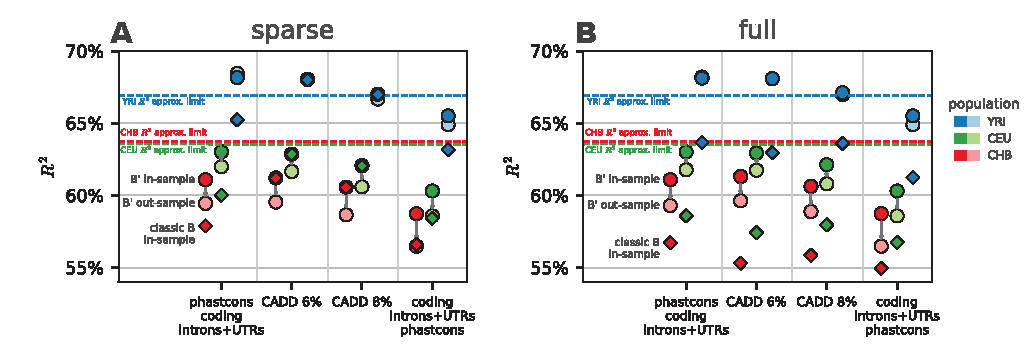
\includegraphics[width=0.8\textwidth]{figures/figure_2.pdf} 

    \caption{Comparison of parameter estimates using classic BGS theory (green
        lines) with our new B' method (blue lines) across both full and sparse
        track types (dark versus light hue), and different mutation rates
        (columns). In the first row, $R^2$ between predictions and observations
        increases with selection intensity. Both classic BGS and B' methods fit
        the data equally well with sparse tracks, though the estimated
        selection coefficients are inaccurate when selection is weak (second
        row). Mutation rate estimates (third row) are more accurately estimated
        by the B' method than classic BGS, but overall show slight biases.
        Overall, classic BGS methods break down as expected when full-coverage tracks
    are used, since it cannot accommodate weak selection and neutrality in putatively
    conserved regions. See methods for details on sparse versus full tracks.
    }

  \label{fig:figure-2}
\end{figure}

Our composite-likelihood method estimates the distribution
of selection coefficients for each feature type, the mutation rate, and the
diversity in the absence of linked selection ($\pi_0$) by fitting the theoretic
reduction map to windowed genome-wide diversity (see Methods
\nameref{sec:methods-likelihood}). We validated that our method can accurately
estimate the selective parameters by simulation a ``synthetic
genome" of the first five human chromosomes (see Methods
\nameref{sec:methods-sim}). We note three findings from these simulations.

First, both our implementation of classic BGS theory and our B' method
accurately infer the average selection coefficient under strong selection
(Figure \ref{fig:figure-2}, middle row). However, when selection was weak, the
classic BGS model erroneously estimated strong selection and a very low
mutation rate. By contrast, our B' method estimated selection coefficients much
more accurately. A minor discrepancy occurs around $2Ns = 1$, likely
due to the sensitivity of mutations in this region to selective interference
(these results do not use local rescaling). 
To ease computational costs, we only simulated fixed selection coefficients and five chromosomes, 
and we only assessed the accuracy of average selection coefficients rather than the full estimated DFE.

Second, we find slight biases in mutation rate estimates from both our B' and the
classic BGS methods (Figure \ref{fig:figure-2}, bottom row). However, mutation
rate estimates based on our B' method are more accurate than classic BGS theory
across a range of selection coefficients. Overall, the bias in estimated
mutation rates suggests that benchmarking genome-wide negative selection models
based on their agreement with pedigree-based rate estimates may not be
appropriate. When BGS is not occurring, either due to weak selection or a low
rate of deleterious mutations (Figure \ref{fig:figure-2}, right column), all
estimates deteriorate. This is understandable, as the overall signal from
linked selection weakens relative to drift-based noise. We should note, though,
that this is an unlikely region of parameter space and this issue can be
readily diagnosed from the low $R^2$ values. Finally, we find in additional
tests that our estimates are robust to demographic expansions but inaccurate
when mutations have recessive effects, since our model assumes additive
effects (see Supplementary Materials Section \ref{supp:sim-assum}). We did not
test the influence of population bottlenecks, since parameter estimates of
out-of-Africa bottlenecked populations (CHB and CEU) did not differ much from
YRI estimates (see below).

Third, we find the coefficient of determination, $R^2$, between predicted and simulated megabase-scale diversity serves as a measure of the strength of the linked selection signal in genome-wide data. $R^2$ increases with the intensity of selection against new deleterious mutations and mutation rate (Figure \ref{fig:figure-2}, top
row). Under just drift or weak purifying selection, the variance in diversity is
driven by unstructured coalescence noise along the genome and the predicted
reduction map, $B(x)$, and does not fit the data well. Under very strong selection
($s=0.05$), $R^2$ is reduced; this is likely due to very strong selection
having less localized effects and impacting overall genome-wide diversity
\parencite{Santiago1995-hx,Robertson1961-ho}.


\subsection*{Application to Human Genomic Data}

\subsubsection*{Annotation Model Comparison}
\label{sec:annotation}

Our composite likelihood method takes tracks of annotated features (an
``annotation model") that are \emph{a priori} expected to have similar fitness
effects, and estimates the overall mutation rate and distribution of fitness
effects for each feature type. We consider two classes of annotation models:
(1) CADD-based models, which consider the top $x\%$ most pathogenic basepairs
according to the CADD score, and (2) and more interpretable, feature-based
models that includes protein coding regions, introns and UTRs, and PhastCons
regions. We include PhastCons regions because they include 
highly-conserved, non-coding regions known to harbor important functions
\parencite{Meader2010-hm,Harmston2013-tt,Katzman2007-gq,Siepel2005-wh}, that
would be missed by gene feature only annotation. These two classes of
annotation models have a trade-off between fine-scaled specificity to which
basepairs are likely to be under negative selection, and interpretability of
the DFE estimates for each feature.

Our method estimates a distribution of fitness effects (DFE) for each feature
class. While CADD-based models only have a single conserved feature class (e.g.
CADD 6\%), feature-based models can have multiple feature classes under varying
levels of selective constrain. However, overlapping features (e.g. a basepair
that is annotated as both PhastCons and coding sequence) must be assigned to
one category or the other. Since this assignment impacts DFE estimates, we fit
both of the two alternative models. First, a \emph{PhastCons Priority} model,
where genic features that overlap PhastCons regions are classified as
PhastCons, and all remaining coding basepairs are labeled as CDS. Second, a
\emph{Feature Priority} model, where all coding basepairs are assigned to CDS,
and the PhastCons class catches the remaining highly-conserved non-genic
regions. 

In total, we fit four annotation models (CADD 6\%, CADD 8\%, PhastCons
Priority, and Feature Priority) to high-coverage 1000 Genome data for three
reference samples: Yoruba (YRI), Han Chinese (CHB), and European (CEU). We assess and compare our models according to how well they predict
patterns of diversity on whole chromosomes left-out during the model fitting
process (e.g. leave-one-chromosome-out, LOCO). We use the metric
$R_\text{LOCO}^2$, which is the proportion of the observed variance in genomic
diversity at the megabase scale predicted by our model on held out data. 
We experimented with a few smaller spatial scales (e.g. 100 kbp), but our results were consistent 
with previous results suggesting the human linked selection signal due to purifying selection
fits best at the megabase scale \parencite{Murphy2022-sj}.

\begin{figure}[htbp] \centering
    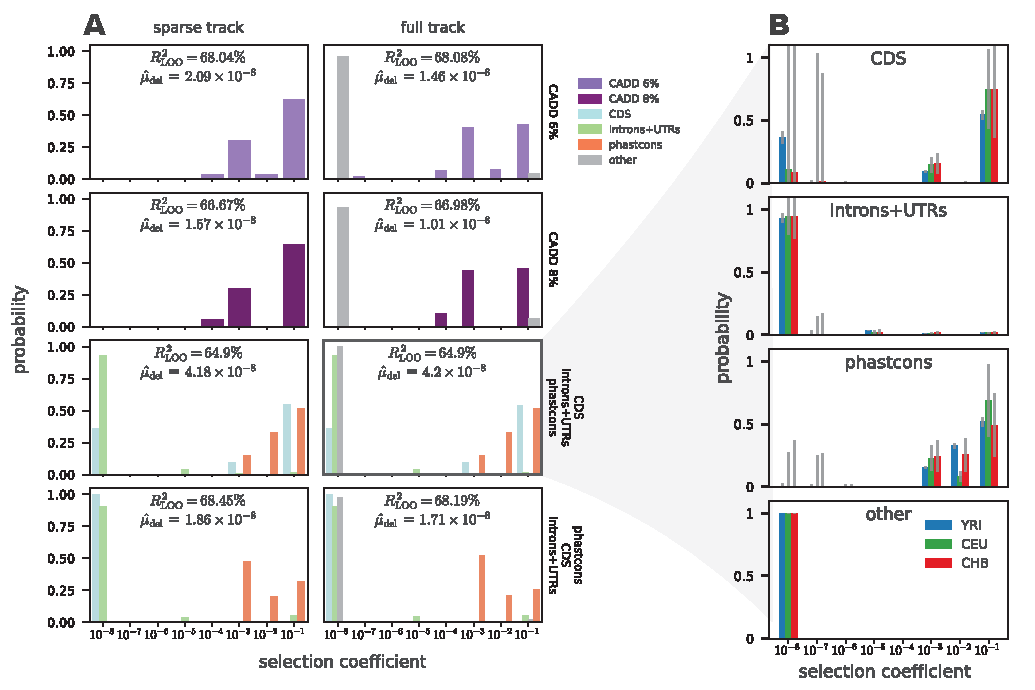
\includegraphics[width=\textwidth]{figures/figure_3.pdf} 

    \caption{The $R^2$ estimates for sparse (A) and full (B) models, for all
        samples (colors) fit at the megabase-scale. Round points are our B'
        method and diamonds are the classic BGS (we exclude classic BGS in the
        full track subfigure, since these all fit very poorly). Lighter color
        round points are the out-sample $R_\text{LOCO}^2$ estimates for our B'
        method, and arrows show the decline in goodness-of-fit due to in-sample
        overfitting (out-sample $R_\text{LOCO}^2$ were not calculated for
        classic B values due to computational costs). The horizontal dashed
        lines are the $R_\text{drift}^2$ expected when the residual variance is
    given by the theoretic variance in coalescence times due to drift alone.}

  \label{fig:figure-3}
\end{figure}

Overall, we find the PhastCons Priority and CADD 6\% models fit equally
well (Figure \ref{fig:figure-2}A), consistent with recent work using classic
BGS theory \parencite{Murphy2022-sj}. However, we find that our models predict
out-of-sample diversity levels slightly better than previous methods. For these
two models, we find that our B' method predicts $R_\text{LOCO}^2=67.3$\% and
$R_\text{LOCO}^2=66.7$\% of the out-of-sample variance in Yoruba pairwise
diversity at the megabase-scale, respectively. By contrast, the best-fitting
CADD 6\% model from \textcite{Murphy2022-sj} explained 60\% of diversity in
left-out 2 Mbp windows across YRI samples. We note that this difference could
be explained by other differences in data processing, optimization, etc. For
lineages impacted by the out-of-Africa bottleneck, the goodness-of-fit was
lower across all models (e.g. 61.0\% and 58.8\% for CEU and CHB respectively in
the PhastCons Priority model).

Since our method is built upon theory that fixes the weak selection problem of
classic BGS theory, it should in principle fit equally well when an annotation
model includes regions that are under no or little selective constraint and thus
(nearly) neutrally evolving. To test this, for each of our annotation models (which are
``sparse") we fit a corresponding ``full" model that assigns the remaining
portion of the genome to a feature called ``other". Ideally, how a model fits
using our B' method should be invariant to whether an annotation model is
sparse or full, since our method in principle can accommodate weak selection
and neutrality. Indeed, we find that both in-sample $R^2$ and
out-of-sample $R_\text{LOCO}^2$ values are nearly identical across full and
sparse-track models (Figures \ref{fig:figure-2}A and \ref{fig:figure-2}B, round
points), which demonstrates that our method is able to deal with weak selection
and that there is little more predictive power to gain from including sites considered ``other'' as annotations. 

By contrast, full annotation models fit poorly under classic BGS theory, and
lead to unreasonable parameter estimates. Additionally, when sparse annotation
models contain genomic features that are likely under weak constraint (such as
introns and UTRs), models fit worse under classic BGS theory than our B' method
(Figure \ref{fig:figure-2}A). However, among the CADD annotation models, the
goodness-of-fit is nearly identical between B' and classic BGS methods. This
behavior is what we would expect given that the CADD models contain only the
most pathogenic sites, which are \emph{a priori} very likely under the strong
selection domain under which B' and classic BGS theory agree.

Overall, our $R_\text{LOCO}^2$ estimates suggest our model
explains up to 67\% of out-sample variance in diversity of the megabase scale,
even though our method assumes constant demography and homogeneous mutation
rates along the genome. A worthwhile question is: how much variation
\emph{could} we expect to fit at this scale? Given that selection alters
genealogies in ways beyond just decreasing mean pairwise coalescence time and
populations have non-constant demography, an exact analytic answer is
intractable. However, we can get an approximate idea if we assume that the
residual variance $\sum_b (\pi_b - \widehat{\pi}_b)^2$ is determined entirely
by the expected neutral coalescence noise around the expected coalescence time
$2B(b)N$. This can be be found analytically, plugging-in our predictions for
$B(b)$. This allows us to calculate $R_\text{coal}^2$ to ballpark the theoretic
variance that is capable of being explained, assuming this coalescent
noise process alone (see Supplementary Materials \ref{supp:r2-coal}). We note that
selection is expected to \emph{decrease} the variance in coalescence times
beyond a rescaled effective population size implies, thus our $R_\text{coal}^2$
would be an underestimate under models with selection.

We find that our out-sample $R_\text{LOCO}^2$ for the Yoruba samples
($R_\text{LOCO}^2 \approx 67$\%) is slightly above the theoretic
$R_\text{coal}^2 \approx 66.6$\%. This suggests our model is in the vicinity of
fitting all the signal possible, under the coalescence-only noise assumption.
By contrast, for bottlenecked out-of-Africa samples, we find a larger
discrepancy between $R_\text{coal}^2$ and observed out-sample
$R_\text{LOCO}^2$. The theoretic $R_\text{coal}^2 \approx 63\%-64$\% for both
samples, compared to the observed $R_\text{LOCO}^2 \approx 61$\% for CEU
and $R_\text{LOCO}^2 \approx 59$\% for CHB under the PhastCons Priority model.
Given that bottlenecks would act to increase the residual variance in
coalescence times beyond the level implied by the effective population size,
this gap would likely shrink under more realistic models or simulation-based
approximations for $R_\text{coal}^2$. Overall, this suggests that purifying
selection models fit the vast majority coalescence time variation at the
megabase-scale that is capable of being explained (i.e. that is not coalescent
noise).

\subsubsection*{Estimated Distribution of Fitness Effects}

\begin{figure}[htbp] \centering
    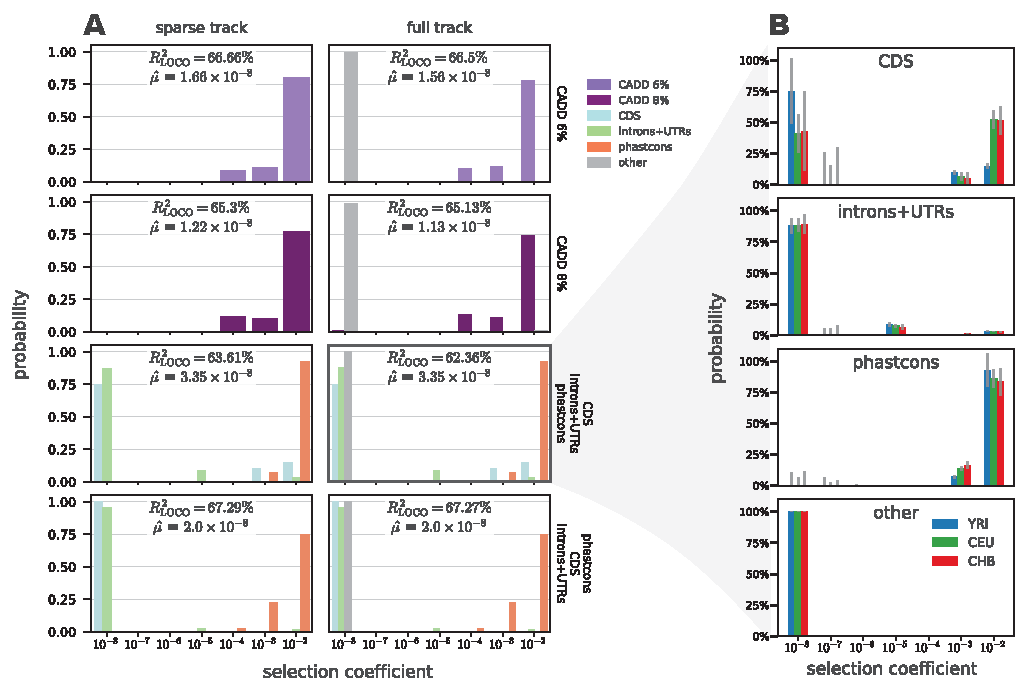
\includegraphics[width=\textwidth]{figures/figure_4.pdf} 

    \caption{The distribution of fitness effects of new mutations estimates for
        YRI reference samples. (A) The DFEs using sparse (left column) and
        full-coverage (right column) tracks, across different annotation models
        (row). Color indicates the feature type. (B) The DFE of the
    full-coverage Feature Priority model comparing the estimates across
reference population samples. Although this model fit the data less well than alternatives, its
results are more interpretable.}

  \label{fig:figure-4}
\end{figure}

Our composite likelihood method has three sets of parameters: the expected
diversity in the absence of linked selection diversity $\pi_0$, the mutation
rate $\mu$, and the matrix of distribution of fitness effects $\mathbf{W}$
across the selection grid for each of the $K$ feature types. Given that the
relationship between $\pi$ and the strength selection is U-shaped (i.e., see \ref{fig:figure-1}A), we wondered
whether our new B' model accommodating weak selection would fit the linked
selection signal under a different combination of weak and strong selection
parameters than observed previously.
However, across all of our annotation models, new deleterious mutations in
conserved feature classes (CADD tracks, CDS, and PhastCons regions) were
consistently estimated to have strongly deleterious effects (Figure
\ref{fig:figure-4}A), consistent with previous work
\parencite{McVicker2009-ax,Murphy2022-sj}. The DFE estimates for CADD and
PhastCons regions consistently places $\ge 75\%$ of mass on the largest
selection coefficient we used, $s=10^{-2}$. The CADD 6\% DFE estimates imply an average
selection coefficient of $\bar{s} = 0.0065$ for CEU, $\bar{s} = 0.0057$ for
CHB, and $\bar{s} = 0.0079$ for YRI. Similarly, the PhastCons Priority model
implies average selection coefficient estimates of $\bar{s} = 0.0063$, $\bar{s}
= 0.0059$, and $\bar{s}= 0.0077$ for CEU, CHB, and YRI respectively for
PhastCons regions. Our DFE estimates for CDS under the Feature Priority model
are qualitatively consistent with the U-shaped DFEs found for amino acids
through Poisson Random Field method \parencite{Boyko2008-tj}.

Following previous work, our method used a grid of selection coefficients up to
$s=10^{-2}$. However, we also experimented with a strong selection grid that
includes $s=10^{-1}$. We find that models fit with the strong selection grid 
have predictive accuracy, as measured with $R_\text{LOCO}^2$, that were about one percentage point higher. This is suggestive of stronger selection than has previously been estimated using
constrained grids (see Supplementary Materials Table
\ref{supp:tbl-r2-strongsel}). For this strong selection grid, we estimate
average selection coefficients for the CADD 6\% model of $\bar{s} = 0.042$ for
CEU, $0.032$ for CHB, and $0.044$ for YRI. Thus, the predefined selection coefficient grid affects ultimate estimates of the DFE and average selection coefficient.


However, we find indications of model non-identifiability across the strong selection grid runs. First, estimates of the DFE with the strong grid are
bimodal (Supplementary Figure \ref{suppfig:strong-sel-dfe}). For
example, under the CADD 6\% strong selection grid model, new mutations are
estimated to have a selection coefficients of $s = 10^{-1}$ with 43\% chance,
$s=10^{-2}$ with 7.8\% chance, and $s=10^{-3}$ with 41\% chance in the YRI
samples. We propose that one mechanism for this non-identifiability is that
very deleterious mutations lead to larger whole-genome reductions in diversity, which are
difficult to distinguish from a smaller drift effective population size (i.e.
the $\pi_0$ parameter). One way to test this hypothesis is to look to see if
there is a systematic positive relationship across models between average
selection coefficient and $\pi_0$, which is includes the drift-effective
population size $N_e$. We find this is the case for all of our CADD 6\% models. Across all reference samples, average selection was about $7.1$ times larger using the strong
selection grid, and $\pi_0$ was $5.6\%$ higher (see Supplementary Materials
Figure \ref{suppfig:sel-ident}). There was no similar consistent change in
mutation rate estimates among reference samples. In the CADD 6\% model, genome-wide
average reduction factor $\bar{B}$ was $\approx 6.1\%$ lower in the default
versus constrained grid. Overall, this suggests that the linked selection
signal alone cannot differentiate very strong selection from a slightly smaller
drift-effective population size. 

Given that it is debated how strongly demography impacts the deleterious
mutation load
\parencite{Torres2018-ni,Torres2020-hc,Lohmueller2008-qi,Simons2014-sv,Simons2016-cs},
we were curious how consistent our DFE estimates are across samples from different reference populations. Overall, we find DFE estimates are relatively stable across samples from different reference populations and annotation models (Supplementary Materials Section \ref{supp:fits}). Only in our Feature
Priority model (Figure \ref{fig:figure-4}B, top row) do we see a slightly
different DFE estimate for coding sequences between YRI and CEU/CHB
samples, but this could be due to the poorer fit this model has to data.

Although the Feature Priority model fits the data less well than alternative
models, its DFE estimates are more interpretable. We find that our B'
method estimates a bimodal DFE for coding sequences for the Feature Priority
model, with a large mass placed on $10^{-3} \le s \le 10^{-2}$ and another on
the neutral class $s=10^{-8}$. This is expected, given that the synonymous and
non-synonymous sites that constitute coding sequences are under vastly
different levels of constraint and are lumped together in our annotation class.
Moreover, features expected to be only weakly
constrained such as introns and UTRs have the bulk of DFE mass on the neutral
class, with a small but significant amount of mass ($\approx 3\%$) placed on
$s=10^{-2}$. As expected, the DFE for PhastCons regions (which in this model
correspond to highly-conserved non-coding elements) suggests it is under strong
selective constraint; however, we note that block jackknife-based uncertainty
estimates suggest the model is uncertain whether there is some mass on the
neutral class. Finally, we highlight one result from our PhastCons Priority
annotation model (Figure \ref{fig:figure-3}A bottom row): the DFE estimate for
coding sequences excluding PhastCons regions is estimated as neutral. This too
is expected; the selection signal in coding regions is absorbed by the
PhastCons feature, leaving only conditionally neutral sites.

\subsubsection*{Estimates of the Deleterious Mutation Rate Are Sensitive to Model Choice}

\begin{figure}[htbp] 
    \centering
    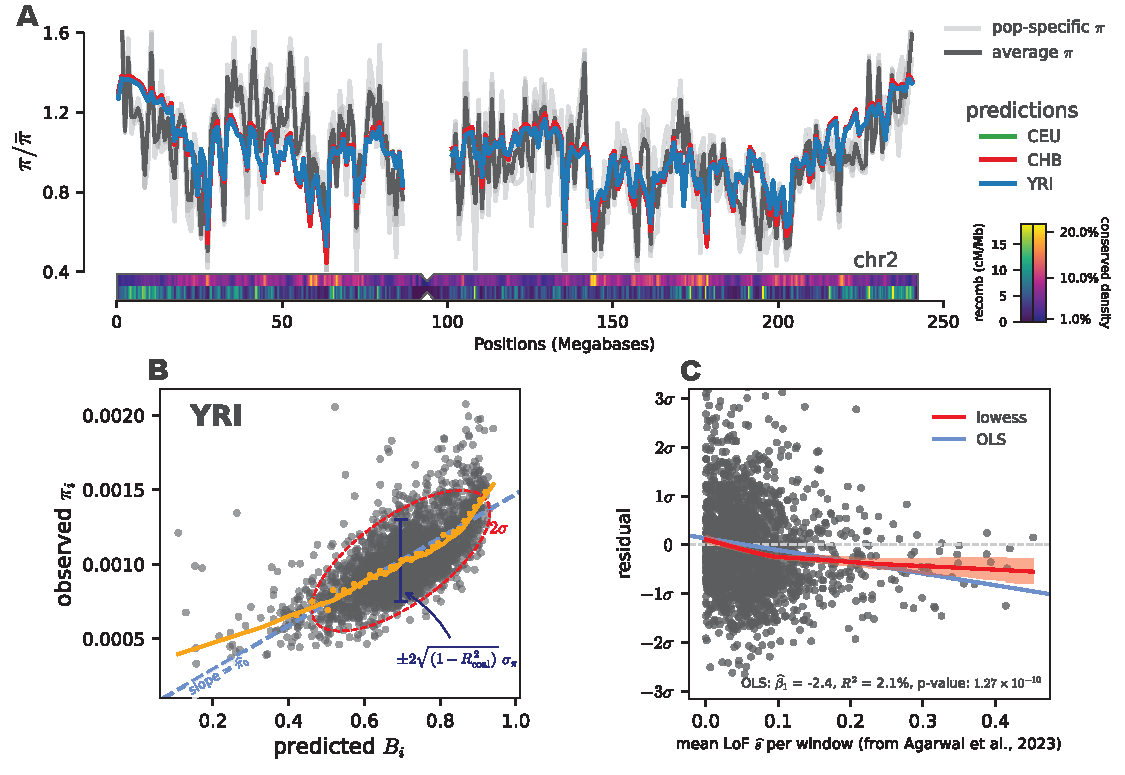
\includegraphics[width=0.5\textwidth]{figures/figure_5.pdf} 
    
    \caption{Mutation rate estimates across the sparse (top row) and
        full-coverage tracks (bottom row) models, for the new B' (circles) and
        classic BGS (diamonds) methods. Estimates of the mutation rate are
        consistent between classic BGS and B' methods for sparse tracks CADD
        models (overlapping diamonds and circles, top row). Overall, mutation
        rate estimates are sensitive to the underlying annotation model.}
  \label{fig:figure-5}
\end{figure}

Prior work on genome-wide inference using the classic BGS model fit the patterns of diversity well,
but led to unusually high estimates of the mutation rate
\parencite{McVicker2009-ax}. This led to the hypothesis that these models
could be absorbing the signal of positive selection \parencite{Enard2014-kz},
though other work has found a limited role for hitchhiking at amino acid substitutions \parencite{Pickrell2009-tt,Hernandez2011-gs,Murphy2022-sj}. While our simulation
results suggest estimates of the mutation rate from linked selection models are
biased, we still check for rough agreement with pedigree-based estimates
\parencite{Kong2013-fc,Tian2019-so}. 
We find across all populations, our mutation rate estimates from CADD-based
models are roughly consistent with pedigree-based estimates (Figure
\ref{fig:figure-4}A), consistent with recent work \parencite{Murphy2022-sj}.
Our full-track CADD 6\% model estimates the mutation rate as $\widehat{\mu} =
1.56 \times 10^{-8}$ for YRI, $1.64 \times 10^{-8}$ for CEU, and $1.60 \times
10^{-8}$ for CHB reference samples (Supplementary Materials Table
\ref{supp:tbl-r2}). As expected, the sparse-track CADD model mutation rate
estimates are nearly identical between the B' and classic BGS methods (Figure
\ref{fig:figure-4}A top row).

However, mutation rate estimates for feature-based annotation models
do not agree with pedigree-based estimates. First, mutation rate
estimates under from classic BGS theory are an order of
magnitude below the expected range (Figure \ref{fig:figure-4}A top row). We
observe similar behavior when we use the classic BGS model to fit full-coverage
annotation models (Figure \ref{fig:figure-4}A bottom row). This behavior is
consistent with classic BGS theory being unable to fit the DFE to features
under weak constraint (e.g. introns, UTRs, and the ``other" feature), and thus must compensate by estimating too low a mutation rate.

Second, we noticed that across all populations and sparse and full tracks, the CADD 6\% model consistently led to slightly higher mutation rates than the CADD 8\%
model (Figure \ref{fig:figure-4}A bottom row; Supplementary Materials Table
\ref{supp:tbl-r2}). This same pattern was observed in Murphy et al. too (2023;
Appendix 1, Figure 16). This behavior suggests a non-identifiability issue
between a slightly higher per-basepair mutation rate and annotation tracks that
contain more conserved sequence. This is expected from theory, since both
classic BGS and SC16 models only depend on mutation rate through the compound
parameter $\mu L$, where $L$ is the length of the conserved segment. Even
though our method is much more robust to the inclusion of non-conserved regions
like introns, we still observe this non-identifiability issue.

Finally, we note that mutation rate estimates from the Feature Priority model are themselves too high ($\widehat{\mu} \approx 3 \times 10^{-8}$), reminiscent of the high mutation rate estimates found under McVicker et al.'s
(\citeyear{McVicker2009-ax}) model. While both our and Murphy et al.'s CADD and
PhastCons-based models alleviate this issue, it is worth considering why this
could occur. We can potentially gain some insight from comparing the estimated mutation rates from our Feature and PhastCons Priority annotation models, which each contain the exact same number of feature basepairs, but whose composition varies based on the priority of overlapping features. That
one of these models is our best-fitting model and the other our worst
indicates that model fits are sensitive to feature classes which themselves have heterogeneous DFEs. CADD-based models fit better in part due to their
fine-scale resolution of selective effects across the genome. While ideally we
would fit a CADD model with different features corresponding to the different
percentiles of pathogenicity, these features are on the basepair scale and thus
too memory-intensive for our method to currently accommodate.

\subsubsection*{Despite Close Fit, Residual Purifying Selection Signal Remains}

\begin{figure}[htbp] \centering
    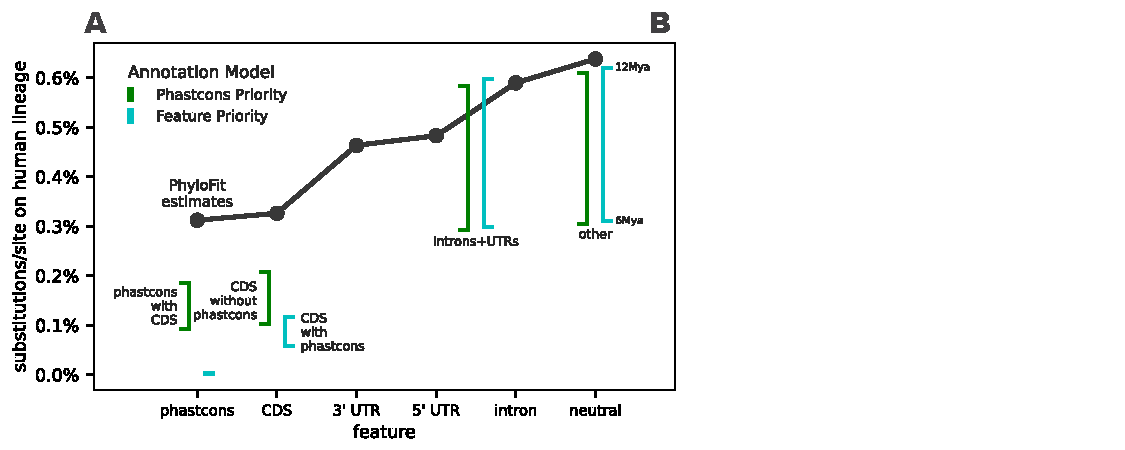
\includegraphics[width=\textwidth]{figures/figure_6.pdf} 

    \caption{(A) Observed and predicted diversity of the B' model fit with the
       CADD 6\% full-track annotation. Once scaled by average diversity, predicted diversity for populations (colored lines) differs little across populations, and closely matches observed diversity within each population (light gray lines). Additionally, we show
        summaries of CADD density and recombination rate along the chromosome
        below. (B) Predicted $B$ and observed $\pi$ for each window. The red dashed line indicates the observed 2 standard deviation ellipsoid, which has nearly the same width as the expected by $R_\text{coal}^2$, indicating the residual variance is close to theoretic expectations. The yellow points are binned means, and the yellow line is the lowess curve through predicted and observed values. (C) CADD 6\% residuals (YRI shown) plotted against the average LoF selection coefficient across genes in megabase windows (estimated by \cite{Agarwal2023-un}).}

  \label{fig:figure-6}
\end{figure}

Comparing predicted against observed diversity along chromosomes, we find a close
correspondence consistent with the high $R_\text{LOCO}^2$ (Figure \ref{fig:figure-5}A). Once scaled by the genome-wide average, predicted and observed diversity levels across the genome differ little across samples from reference populations. Given that the CEU and CHB samples are from bottlenecked out-of-Africa populations and their mutation rate and DFE estimates are similar, this is an empirical demonstration that our model is fairly robust to violations of the constant population size assumption of the theory.

However, we note a few large (tens of megabases) regions with systematically poorer fit
(Supplementary Materials Figure \ref{supp:spatial-residuals}). In Figure
\ref{fig:figure-5}A we see one such region on the short arm of chromosome 2,
from 30 Mbp to 60 Mbp. Interestingly, predicted diversity closely follows the
peaks and troughs of this region, however, predicted diversity is lower than observed. We note that a small region within this stretch had been found by a genome-wide scan for associative overdominance \parencite{Gilbert2020-aw}. We further investigate this by inspecting whether observations are systematically different from predictions. We confirm a finding of \textcite{Murphy2022-sj} that regions predicted to experience little reduction in diversity due to background selection (i.e. $B\approx 1$) have higher diversity than predicted (Figure \ref{fig:figure-5}B, orange line). \textcite{Murphy2022-sj} suggested that this could reflect ancient introgression between archaic humans and ancestors of contemporary humans. Despite the prediction error in this region, the variance around observed and predicted diversity levels falls very close to what we would expect under the theoretic coalescent-noise-only expectation ($R_\text{coal}^2$).

As DFE heterogeneity within a class of sites may be poorly fit by our model,
we looked for unaccounted selection in our model residuals. First, we
inspected whether there was a relationship between the fraction of CADD 2\% and 6\% basepairs and the residual across megabase windows (Supplementary Figure
\ref{suppfig:resid-cadd}), finding a negative significant relationship in
both cases. CADD 2\% was used in this case to search for a residual signal from highly-constrained regions. Moreover, our model over-predicted diversity in windows containing
more CADD 2\% basepairs than CADD 6\%, consistent with heterogeneity in
site pathogenicity being poorly fit by our model. However, the total residual
variance explained is $R^2 = 0.3\%$ and $R^2 = 0.9\%$ for the CADD 2\% and 6\%
tracks respectively, suggesting only a modest amount of selection signal remains within the CADD annotations.

Since our method does not include the possible effects of linked positive
selection, we might expect windows containing hard or soft sweeps would have
systematically lower diversity levels than predicted. Using the locations of
soft and hard sweeps detected using a machine learning approach
\parencite{Schrider2016-xn, Schrider2017-yx}, we tested whether the residuals of the
CADD 6\% model containing sweeps were systematically different than those not
containing sweeps. We find no significant difference between the magnitude of
residuals of windows containing sweeps versus those that do not (Supplementary
Materials Figure \ref{suppfig:resid-sweeps}; Kolmogorov--Smirnov p-value =
0.71). The same was true if we looked at hard or soft sweeps individually as a class. 

We further tested for remaining selection signal in our CADD 6\% model
residuals by using gene-specific estimates of the fitness cost of
loss-of-function (LoF) mutations from \textcite{Agarwal2023-un}. These
estimates are based on an Approximate Bayesian Computation approach that
estimates the posterior distribution over LoF fitness costs from the observed
dearth of LoF mutations per gene, and thus is an independent
approach to assess the strength of purifying selection. We averaged the estimated LoF fitness costs across genes
for each of our megabase windows, and plotted our residuals against these
average LoF fitness costs. Contrary to the weak CADD residual signal described
above, we find evidence of a fairly strong relationship between our residuals
and average LoF fitness cost (Figure \ref{fig:figure-5}C; $R^2 = 2.1\%$,
p-value $1.27 \times 10^{-10}$). In other words, roughly 2\% of the variance in
these residuals is explained by the average fitness costs of LoF mutations in
the window. Consequently, our model over-predicts diversity by about
$\nicefrac{\sigma}{2}$ or more in windows harboring the top 1.7\% most
LoF-intolerant genes.

\subsubsection*{Predicted Substitution Rates Indicate Potential Model Misspecification}

\begin{figure}[htbp] \centering
    \includegraphics[width=\textwidth]{figures/figure_7.pdf} 

    \caption{The divergence implied from predicted substitution rates under the B' model versus observed divergence along the human lineage.
        Black points are the PhyloFit divergence rate estimates per feature
        (on x-axis). Line ranges are the implied divergences across a range of
        human-chimpanzee divergence times of 6-12 Mya (using a generation time of
        28 years). We show the predicted divergences for our Feature
        (turquoise) and PhastCons priority (green) annotation models.
        Additionally, we show the predicted PhastCons region divergences when
    local rescaling is applied (blue; we omit other locally rescaled predictions
since these to not differ substantially).}

  \label{fig:figure-7}
\end{figure}

Since our B' method also predicts deleterious substitution rates ($\widehat{R}$) for each feature class, it allows for another check of model sufficiency by comparing the predicted substitution rates to observed levels of divergence. We estimated sequence divergence on the human lineage using a multiple
alignment of five primates for each feature in our feature-based models
(Methods Section \nameref{sec:methods-sub}). We compared these to the predicted substitution rates per feature, averaging over all segments in the genome. Since our simulations show that mutation rate estimates can be biased, we predicted substitution rates under a fixed mutation rate of $\mu = 1.5 \times
10^{-8}$. Fixing the mutation rate also allows us to more easily compare the
predictions across our feature-based models. Unfortunately, a careful
comparison between our predictions and observed divergence rates is hindered by considerable uncertainty in the rate of the molecular clock, generation times, and the human-chimpanzee divergence time. We assume a generation time of 28 years \parencite{Fenner2005-yi}, and calculate the sequence divergence implied by our predicted
substitution rates over a range of divergence times, from 6 Mya to 12 Mya
\parencite{Moorjani2016-tb,Nachman2000-te,Yi2002-pw,Steiper2006-xx}.

We find that predicted substitution rates are qualitatively consistent with the observed divergence along the human lineage for all features except
the PhastCons regions (Figure \ref{fig:figure-6}). As expected, the predicted substitution rates in features under reduced selective constraint (introns and UTRs, and the ``other" feature) are very close to the mutation rate. Throughout, we report our substitution rates as a percent relative to the total mutation rate, $\mu$ (here fixed to $1.5 \times 10^{-8}$). In our Feature Priority model, coding sequences are predicted to have a substitution rate of 41.20\% of the mutation rate, introns and UTRs 94.71\%, PhastCons regions 0\%, and the ``other" feature 99.98\%. For comparison, the substitution rates along the human lineage
(as a proportion to the substitution rate in putatively neutral regions) are
74.15\% in UTRs, 92.44\% in introns, 50.96\% in coding sequences, and 49.56\%
in PhastCons regions. The large discrepancy between predicted and observed
PhastCons substitution rates is driven by our DFE estimates suggesting that the bulk of mass is on selection coefficients greater than $10^{-3}$, which have no chance of fixation in a population of $N_e \approx 10,000$. We note that our DFE estimates are qualitatively similar to those inferred using the classic BGS model, so the disagreement between observed divergence and predicted substitution rates could indicate a potential model misspecification problem.

\subsubsection*{Possible Signal of Selective Interference}

Given the prediction error for substitution rates in highly-conserved regions and that simulation indicates that $B(x)$ is more accurately predicted when we use local rescaling, we modified our composite-likelihood method so that it can be run a second time, on B' maps locally rescaled by the predicted $\widehat{B}(x)$ from the initial fit. Intuitively, this is based on the notion that if a neutral allele experiences a fitness-effective population size of $B(x)N$, so too should a selected allele, and this should be considered in how the SC16 equations are solved.

There are five important but tentative results to draw from this analysis.
First, estimated mutation rates are in general higher. Under the CADD 6\%
model, they are $\widehat{\mu} = 6-7.3 \times 10^{-8}$ across populations; for
the PhastCons Priority model, they reach the upper limit of our optimization
boundary of $\mu = 8 \times 10^{-8}$ (Supplementary Material
\ref{supp:locally-rescaled-fits}). Second, all of our leave-one-chromosome-out
$R_\text{LOCO}^2$ are about one percentage point higher than the unrescaled
model. Third, the DFE estimates for both CADD 6\% and PhastCons regions in the
PhastCons Priority model is now U-shaped (Supplementary Materials Figure
\ref{suppfig:rescale-dfe}), with $70-77\%$ of mass being placed on a weakly
deleterious class, $s=10{^-5}$. Interestingly, this is the first of all of our
models where such an appreciable mass has been placed on a midpoint in our
selection coefficient grid; in all other cases, non-strongly estimates were
neutral ($s=10^{-8}$). Fourth, predicted pairwise diversity is nearly identical to our original, non-rescaled fit (see Supplementary Materials Figure \ref{suppfig:rescale}). Finally, since local rescaling increases the DFE mass over $s < 10^{-3}$, mutations in PhastCons regions now have the possibility of fixation. We find that local rescaling the PhastCons Priority, leads the predicted substitution rates in PhastCons regions to be much closer to observed levels (blue line, Figure \ref{fig:figure-6}).

Finally, we note an important caveat about this analysis. Since local rescaling is done using the first round of maximum likelihood estimates, there is some possibility of statistical ``double dipping'', since the $B(x)$ at this position includes the contribution of the focal segment that is being rescaled. Ideally, one would exclude this segment's contribution to $B(x)$; however, this is computationally unfeasible. However, two observations indicate our findings here are relatively
robust despite this limitation. First, the results do not change based on
whether the $B(x)$ is averaged at the 1 kbp level or at the megabase scale; for the latter, a single segment makes little contribution to the average. Second, we investigated the extent to which local rescaling modified the B' maps across selection parameters. We find minor differences between the locally rescaled and standard B' maps for fixed selection coefficients (i.e. before model fitting) in the nearly-neutral domain ($0.2 \le 2N_e s \le 2$). Additionally, the locally rescaled and standard maps are identical under strong selection ($2N_e s= 20$) as expected (Supplementary Materials Figure \ref{suppfig:rescale-b}). Moreover, the correlations between the standard and locally rescaled B' maps across the genome are high (100\% for $2N_e s = 20$, 96.5\% for $2N_e s = 2$, and 60.21\% for $2N_e s = 0.2$). The overall realized effect of local rescaling is to just alter how deep the ``U" is in the relationship between the reduction factor $B$ and the selection coefficient (Supplementary Materials Figure
\ref{suppfig:rescale-effects}).

Overall, this suggests that models of the signal of linked selection are worryingly sensitive to the theoretic B' values in the $2Ns \le 1$ domain. The fact that predicted diversity differs little between standard and locally rescaled B' methods indicates there may not be enough information in pairwise diversity alone to differentiate when interference is occurring or the causes of fitness variance along the genome. Moreover, local rescaling turns out to only slightly alter the B' maps, yet significantly modifies the DFE estimates. This brings the deleterious substitution rate in agreement with observations (since this is predicted with a fixed $\mu = 1.5 \times 10^{-8}$; however, the maximum likelihood estimate of mutation is implausibly high. This suggests either the local rescaling approximation to interference is not suitable (though our chromosome-wide simulations show locally rescaled B' maps are close to the reductions observed from simulations), or that the deleterious mutations-only model does not adequately describe the processes generating fitness variance.

\section*{Discussion}

New mutations at functionally important regions of the genome are a major source of fitness variation in natural populations, as the vast majority of such mutations are deleterious. Purifying selection, working to remove these deleterious variants, perturbs genealogies at linked sites, creating large-scale patterns in genomic diversity. While this has been recognized for decades (e.g., \textcite{Nordborg1996-nq,Hudson1995-xc}), the availability of genomic data allows for methods to estimate the degree to which purifying selection shapes genomic variation and at what scale.

Accordingly, there have been a number of recent efforts to fit parametric models of linked selection to polymorphism and divergence data in Drosophila \parencite{Elyashiv2016-vt} and humans \parencite{McVicker2009-ax, Murphy2022-sj}. These efforts have yielded reasonable estimates of the strength of selection on new mutations as well as provided mutation rate estimates that largely agree with pedigree-based estimates. However, previous methods have relied on the canonical background selection model, which assumes that mutations are sufficiently deleterious such that they cannot fix. Consequently, statistical methods using the BGS model should only be expected to fit well when some regions are \emph{a priori} under strong selective constraint. In reality, the relationship between neutral diversity levels and the strength of selection from purifying selection in linked regions is U-shaped, which implies there could be more uncertainty than previously appreciated in the distribution of weak and strongly deleterious mutations.

In this work, we developed and fit a different class of linked selection models based on the equilibrium fitness variance \parencite{Santiago1998-bs,Santiago2016-mu}. Fundamentally, we model the reduction in diversity as a 
function of how additive fitness variance is distributed along the recombination map of the genome \parencite{Santiago1998-bs}. We fit a specific model for this fitness variance that supposes all 
variation is the result of selection against new additive deleterious mutations \parencite{Santiago2016-mu}. 
Unlike classic background selection theory \parencite{Charlesworth1993-gb,Nordborg1996-nq,Hudson1995-pt,Hudson1995-xc}, 
the SC16 model explains equilibrium fitness variance across all selection coefficients by jointly predicting another central quantity in evolutionary genomics: the 
substitution rate of deleterious alleles.

Our method has at least four improvements over previous whole-genome linked selection methods based on the BGS model. First, our model leads to better fits to data than those based on classic BGS, as measured by predicted out-of-sample diversity. Second, unlike BGS-based methods, our model is capable of fitting weak selection. When regions under weak or little selective constraint are included in methods using classic BGS, parameter estimates can become severely biased. By contrast, we have demonstrated via simulation that our method can estimate the strength of selection even for weakly constrained features (e.g. introns and UTRs), as well as remaining unannotated regions of the genome. Third, fitting our model produces a simultaneous prediction of substitution rates, which can be compared to observed divergence rates. Finally, the effect of selective interference can be approximated by locally rescaling the B' maps, which our forward simulations show reduce prediction error of genome-wide diversity levels.

Even though our model is able to fit weak selection, our initial estimates of mutation rate and DFEs were consistent with prior work \parencite{Murphy2022-sj}. This, at first glance, suggests further confirmation that strong purifying selection is the dominant mode of linked selection in the genome. However, we find that predicted substitution rates for highly-conserved PhastCons features disagree with observed rates of divergence along the human lineage. This disparity between observed divergence and predicted substitution rates is likely a consequence of our DFE estimate for PhastCons regions containing little mass over weakly deleterious and neutral selection coefficients that would have some possibility of fixation --- a characteristic of DFE estimates from other work too \parencite{Murphy2022-sj}.

Our simulation results reveal another possible source of disagreement: in the weak selection domain of $2N_e s \approx 1$ there is an appreciable level of disagreement between theory and simulation. We hypothesize that this could be because as $2N_e s$ approaches $1$, a segment under
selective constraint experiences a local fitness-effective population size of $B(x)N$, and not just $N$. This local fitness-effective population size is induced by selection at other segments that is not being taken into account by classic BGS theory or our standard SC16 model. When we experimented by fitting our model and then using the predicted reduction map to locally rescale $N_e$ to the fitness-effective population size $N_f = \widehat{B}(x)$, we found the disagreement between predicted and observed substitution rates disappears. This is expected since locally rescaled DFE estimates have an appreciable mass on weakly deleterious selection coefficients, contrary to the standard fits.

This pattern is consistent with a scenario where the same selection processes that reduce diversity over long stretches along the chromosome also decrease the efficacy of purifying selection. This idea has been proposed before in an extension to the McDonald--Kreitman test that accounts for how 
background selection can bias estimates of the proportion of adaptive substitutions 
\parencite{Uricchio2019-wp}. While our simulation results indicate local rescaling reduces error in the weak selection domain, it is worth noting some caveats about this approach. First, local rescaling is only an approximation to selective interference; as our simulations show, this approximation reduces error in the predicted reduction $B(x)$, but this may not fully account for how negative linkage disequilibrium builds up and reduces fitness variance. A benefit of the SC16 approach is that the equations 
can be solved with a locally rescaled effective population that approximates this process. Second, there is the possibility of circularity, since a preliminary fit must be made to estimate $B(x)$, which is then 
used to re-solve the SC16 equations with a local fitness-effective population size.

Despite these caveats, the local rescaling approach suggests selective interference could alter inferences about the DFE and bring predicted substitution rates into agreement with observed divergence rates.  However, these results also demonstrate that parameter estimates are extremely sensitive to how accurate the theoretic B' maps 
are in this domain. Moreover, we find that predicted diversity differs little across DFE and mutation rate estimates, suggesting there may be limited information in pairwise diversity to differentiate between models, thus inclusion 
of allele or haplotype frequency information might be informative in the future. While local rescaling brings substitution rates into agreement, it also re-introduces a similar problem found by \textcite{McVicker2009-ax}: the 
estimated mutation rate is too high. While our mutation rate includes point mutations as well as all other forms of 
deleterious variation (e.g. insertions/deletions, copy number variants, etc.), our estimations suggest exceedingly high 
rates of deleterious variation per generation.

Examination of the local residuals of our predicted diversity levels demonstrated no systematic effect of previously identified hard and soft selective sweeps \parencite{Schrider2017-yx}. 
This result echoes what has been observed in previous efforts to look at genome-wide patterns of 
linked selection \parencite{Hernandez2011-gs, Murphy2022-sj}, and suggests that the scale of perturbation due to selection sweeps is more restricted (e.g. at the kilobase scale, \cite{Akey2004-zg}) than the scale at which we are modeling variation. Taken together this suggests that selective sweeps are not likely responsible for shaping the 
majority of variance in large-scale patterns of chromosomal variation in humans. 

Given that our model is essentially parameterized by levels of fitness 
variance along the genome, the high estimates of mutation rate could suggest that purifying selection is not the only source of fitness variance generating the genome-wide linked selection signal in humans. 
Selection on polygenic traits could be another source of fitness variance. Alternatively, purifying selection could be the main source of fitness variance, but the complexity of selective interference may be poorly approximated by the local rescaling approach. Another possibility is that our assumption throughout of additive effects may lead to biases given deleterious mutations likely recessive effects. Future theoretic work, as well as realistic across-species forward simulations of multiple modes of linked selection (e.g. \cite{Rodrigues2023-rj}) are needed to fully disentangle these processes. As we find evidence of strong selection against loss-of-function in our model residuals, it is also possible that the bulk of fitness variance \emph{is} due to purifying selection, but our model is unable to account for strong heterogeneity in the DFE per annotation class.

Moving forward it remains a central goal to understand how the sources of fitness variation shape the striking patterns of diversity along the human genome. Our work embeds this question in the quantitative genetic framework that is more accurate and flexible than proceeding models, but there is much work yet to do to incorporate important population genetic features such as dominance effects and selective interference. Overall, the complex interplay of mutation, selection, drift, and interference may confound our understanding of selection in the human genome for some time.

\section*{Acknowledgments}

We would like to thank Doc Edge, Ben Good, Taylor Kessinger, Graham McVicker, Priya Moorjani, Rasmus Nielsen, Guy Sella, Joshua Schraiber, and Peter Sudmant for helpful discussions, and Martin Kircher for providing modified CADD tracks. We thank Graham Coop, Matt Hahn, Nate Pope, and Enrique Santiago for comments on the manuscript.
This research was supported by NIH awards R35GM148253 and R01HG010774 to ADK

\section*{Methods}

\subsection*{Solving the B' Equations for each Segment}
\label{sec:methods-bprime-eqns}

Our software \texttt{bgspy} first calculates the equilibrium additive genic
fitness variation $\widetilde{V}_a$ and deleterious substitution rate $\widetilde{R}$ for each
user-specified segments in the genome. These equilibria are calculated across
grids of mutation rate weighted by the DFE $m_i$ and selection coefficient
$s_j$, by numerically solving the following system of equations,

\begin{align}
  \label{eq:method-2eqns}
  {N}_f &= N \exp \left( -V_a \frac{Q^2(m_i, s_j)}{2} \right) & \text{\emph{effective population equation}} \\
  R &= \frac{4N_fU s_j}{\exp(4 N_f s_j)-1}  & \text{\emph{substitution equation}} 
\end{align}

where,
%
\begin{align}
  %V(x) &= U s - 2 {R}(x) s & \text{\emph{fitness variance equation}} \\
  V_a &= (U - 2 R) s_j & \text{\emph{fitness variance equation}} \\
  Q^2(m_i, s_j) &= \frac{2}{(1-Z)(2-(2-M)Z)} & \text{\emph{linkage inflation factor}} \\
  Z &= 1 - \frac{Us_j}{U-{M}} & \text{\emph{variance decay rate}}
\end{align}
%
and $U = m_i L$ and $M = r_\text{BP} L$ are the total mutation and
recombination rates in the segment. A detailed derivation of these equations
can be found in Supplementary Materials Section \ref{supp:theory}. The recombination
rate in a segment is determined by a user-supplied recombination map.

\subsection*{Calculating the Reduction Maps}
\label{sec:methods-maps}

Our method uses the pre-computed equilibria $\widetilde{V}_{a,g}$ for each
segment $g$ to calculate the reduction map $B(x; m_i, s_j)$ at positions $x$
across the parameter grids described above. Since we assume multiplicative
fitness, the reduction is the product of each segment's contribution accounting
for the recombination is,

\begin{align}
    B(x; m_i, s_j) = \exp\left(- \frac{1}{2}\sum_{g \in G} \sum_{i=1}^{n_s} \widetilde{V}_{a,g}(m_i, s_j) Q_g^2(m_i, s_j, r_{x, g})\right)
\end{align}
%
where $r_{x, g}$ is the recombination fraction between the focal site and
segment $g$. Here, $Q^2(m_i, s_j, r_{x,g})$ is given by Equation \eqref{eq:Q}
squared. A separate reduction map is calculated for all features $G$ within a
specific feature type. We calculate B' calculate for $\log_{10}$-spaced grids
over $10^{-1} \le s \le 10^{-8}$ and $10^{-11} \le m \le 10^{-7}$, in 10kb
increments across the genome.

\subsection*{Composite Likelihood and Optimization}
\label{sec:methods-likelihood}

Following previous approaches
\parencite{McVicker2009-ax,Elyashiv2016-vt,Murphy2022-sj}, we use a composite
likelihood approach to fit our negative selection model. Per-basepair allele
count data (described below) is summarized into the number of same and
different pairwise differences per window. All of our primary models were fit
with megabase windows, since previous work has found the strongest selection
signal at this scale (we confirm this with one CADD 6\% fit at the $100$ kbp
scale).

Our binomial likelihood models the number of different pairwise comparisons
observed per window given the total number of pairwise comparisons. The
binomial probability for window $b$ is $\bar{\pi}(b; \Psi) = \pi_0 \bar{B}(b;
\mu, \mathbf{W})$, where bars indicate averages over some bin width. The free
parameters $\Psi = \{\pi_0, \mu, \mathbf{W}\}$ are the expected diversity in
the absence of selection ($\pi_0$), the mutation rate ($\mu$), and the
distribution of fitness effects for the discretized selection grid and $K$
features ($\mathbf{W}$). The reduction at position $x$ is then,

\begin{align}
    \log\left(B(x; \mu, \mathbf{W}) \right) = - \frac{1}{2} \sum_{g \in G} \sum_{j=1}^{n_s} V_g(\mu W_{j, k(g)}, s_j) Q_g^2(m_i, s_j, r_{x, g}).
\end{align}
%
See Supplementary Materials Sections \ref{supp:data-summary} and
\ref{supp:likelihood} for more details.

Our method uses two tricks to improve optimization over the mutation and DFE
parameters. First, we find $B(x; \mu, \mathbf{W})$ is exponential over columns
of $\mu \mathbf{W}$, which allows for optimization over this smooth function
rather than the grid. Second, we use softmax to convert constrained
optimization over the DFE columns (which must sum to one) to unconstrained. We
tested multiple different optimization routines, finding that BOBYQA
outperformed alternatives \parencite{Powell2009-jm,Johnson2007-tl}. We
inspected and confirmed convergence with diagnostic plots finding stable optima
across 10,000 random starts (see Supplementary Materials Section
\ref{supp:optim}). We assessed model fit using out-sample predictive error,
calculated by leaving out a whole chromosome during fitting and predicting its
diversity. To calculate uncertainty, we used a block jackknife approach in 10
Mbp windows (Supplementary Materials Section \ref{supp:jackknife}).

\subsection*{Human Population Genomic Data}
\label{sec:methods-data}

Our analyses was conducted on the Yoruba (YRI), European (CEU), and Han Chinese
(CHB) reference sample individuals from the high-coverage 1000 Human Genomes
data aligned to GRCh38/hg38 \parencite{Byrska-Bishop2022-tn}. Since nucleotide
diversity is a ratio estimator, it can be biased when subtly different
filtering criteria are applied to variant and invariant sites. To prevent this,
we conducted our analyses on Genomic VCF (gVCF) files that contain genotype
calls for both variant and invariant sites \parencite{Illumina_Inc2020-dk}.
Then, we apply the same genotype filtering criteria to all called sites
(Supplementary Materials Section \ref{supp:filter}). We also applied sequence
accessibility masks that containing only non-repeat, non-centromeric sequence
that passed the 1000 Genomes strict filter
(\cite{1000_Genomes_Project_Consortium2015-mi}; Supplementary Material Section
\ref{supp:accessible}). Since our theory only considers the indirect effects of
linked selection on a site, we additionally masked sites that are likely under
direct selective constraint (see Supplementary Materials Section
\ref{supp:neutral}). Finally, for every basepair passing these filtering and
masking criteria, we counted the number of reference and alternative allele
counts (excluding all multiallelic, indel, and CNV variants).

For all of our main analyses, we used the recombination map from
\textcite{Halldorsson2019-ey} estimated from a trio-based design to avoid
circularity that could occur by using LD-based maps. We use Ensembl gene
annotation \parencite{Cunningham2022-vk}, a special CADD Score dataset with
McVicker B scores removed (to avoid circularity;
\cite{Kircher2014-bv,Rentzsch2019-lr}), and PhastCons regions
\parencite{Siepel2005-wh}. We did not account for mutation rate heterogeneity
along the genome, since this would require using divergence-based estimates of
local mutation rates that would introduce circularity when we predict
divergence rates under our model.

\subsection*{Forward Simulations}
\label{sec:methods-sim}

We conducted forward simulations of negative selection on whole human
chromosomes to validate our method at two stages. First, we simulated negative
selection on chromosome 10 using a realistic recombination map and putatively
conserved features to confirm that our classic B and new B' maps matched the
average simulation reduction map across mutation and selection parameters.
Second, we evaluated our composite likelihood method by simulating negative
selection on the first five human chromosomes, across grids of fixed mutation
and selection parameters. We then combined these into a synthetic genome, and
overlaid mutations on the ARG. Then, we ran our likelihood methods on the
resulting allele count data to assess model accuracy. We ran additional
synthetic genome simulations like these to evaluate the impact of two model
violations: recessivity of deleterious mutations and expanding populations. For
the latter, after $9.3$ generations, we grew the population by factor of 1.004
each generation to mimic the human expansion out-of-Africa
\parencite{Gutenkunst2009-pg}. We did not simulate population bottlenecks since
our analyses showed little difference between bottlenecked out-of-Africa
samples (CEU and CHB) and YRI samples. More details about these and the segment
simulations shown in Figure \ref{fig:figure-1}A-C can be found Supplementary
Materials Section \ref{supp:simulation}.

\subsection*{Substitution Rate Prediction and Divergence Estimates}
\label{sec:methods-sub}

Substitution rates were predicted by resolving Equations \eqref{eq:main_eqns} for the given estimated product between mutation rate and DFE weight, $w_{i,j} = \mu W_{i,j}$. We estimated the divergence along the human branch using PhyloFit
\parencite{Siepel2004-ql} run on a subset of the UCSC 17-way Multiz alignments
\parencite{Blanchette2004-bb} consisting of humans and four other primates (\emph{Pongo
abelii}, \emph{Pan troglodytes}, \emph{Pan paniscus}, \emph{Gorilla gorilla}).
PhyloFit was run using the HKY85 substitution model per-feature; estimates from
alternate substitution models yielded equivalent results. Further details about
this process can be be found in the GitHub repository
(\url{https://github.com/vsbuffalo/bprime}). 
\subsection*{Data Availability}

All code from \texttt{bgspy} and our Jupyter Lab \parencite{Kluyver_undated-ol}
notebooks for analysis are available on GitHub
(\url{https://github.com/vsbuffalo/bprime}). The main model fits are available
as Python Pickle objects on Data Dryad repository (\url{https://doi.org/10.5061/dryad.qnk98sfnv}).

\printbibliography

\end{document}
